\documentclass[11pt,twoside]{book}
\usepackage[mono=false]{libertine} % new linux font, ignore mono
\usepackage{luatex85}

\usepackage{amsmath,amsthm,amssymb,mathrsfs,amsfonts,dsfont}
\usepackage{epsfig,graphicx}
\usepackage{tabularx}
\usepackage{blkarray}
\usepackage{slashed}
\usepackage{color}
\usepackage{listings}
\lstset{
    language=bash,
    basicstyle=\ttfamily,
    breaklines=true,
    showstringspaces=false,
    commentstyle=\color{green!40!black},
    keywordstyle=\color{blue},
    stringstyle=\color{orange}
}
\usepackage{caption}
\usepackage{lipsum} % provides dummy text for testing
\usepackage[toc,title,titletoc,header]{appendix}
\usepackage{minitoc}
\usepackage{multicol} % two-col ToC
\usepackage{bm}
\usepackage{imakeidx} % before hyperref
\usepackage{hyperref}
\hypersetup{
    colorlinks=true,
    citecolor=magenta,
    linkcolor=black,
    filecolor=green,      
    urlcolor=cyan,
}
\usepackage[capitalise]{cleveref}
\usepackage{subcaption}
\usepackage{enumitem}
\usepackage{mathtools}
\usepackage{physics}
\usepackage[linesnumbered,ruled,vlined,algosection]{algorithm2e}
\SetCommentSty{textsf}
\usepackage{epigraph}
\epigraphwidth=1.0\linewidth
\epigraphrule=0pt

% adjust margin
\usepackage[margin=2.3cm]{geometry}
\headheight13.6pt

\usepackage{fancyhdr}
\pagestyle{fancy} % enable fancy page style
\renewcommand{\headrulewidth}{0.0pt} % comment if you want the rule
\fancyhf{} % clear header and footer
\fancyhead[lo,le]{\leftmark}
\fancyhead[re,ro]{\rightmark}
\fancyfoot[CE,CO]{\hyperref[toc-contents]{\thepage}}

\makeatletter
\def\chaptermark#1{\markboth{\protect\hyper@linkstart{link}{\@currentHref}{Chapter \thechapter ~ #1}\protect\hyper@linkend}{}}
\def\sectionmark#1{\markright{\protect\hyper@linkstart{link}{\@currentHref}{\thesection ~ #1}\protect\hyper@linkend}}
\makeatother

\usepackage[doi=false,url=false,isbn=false,style=alphabetic,backend=biber,backref=true]{biblatex}
\addbibresource{bib.bib}

\newbibmacro{string+doiurlisbn}[1]{%
  \iffieldundef{doi}{%
    \iffieldundef{url}{%
      \iffieldundef{isbn}{%
        \iffieldundef{issn}{%
          #1%
        }{%
          \href{http://books.google.com/books?vid=ISSN\thefield{issn}}{#1}%
        }%
      }{%
        \href{http://books.google.com/books?vid=ISBN\thefield{isbn}}{#1}%
      }%
    }{%
      \href{\thefield{url}}{#1}%
    }%
  }{%
    \href{http://dx.doi.org/\thefield{doi}}{#1}%
  }%
}

\DeclareFieldFormat[article,incollection,inproceedings,book,misc]{title}{\usebibmacro{string+doiurlisbn}{\mkbibemph{#1}}}
\DeclareFieldFormat{journaltitle}{#1\isdot}
\DeclareFieldFormat{booktitle}{#1\isdot}
\renewbibmacro{in:}{}
\DeclareSourcemap{
    \maps[datatype=bibtex]{
      \map{
        \step[fieldsource=video]
        \step[fieldset=usera,origfieldval]
    }
  }
}
\DeclareFieldFormat{usera}{\href{#1}{\textsc{Online video}}}
\AtEveryBibitem{
    \csappto{blx@bbx@\thefield{entrytype}}{% put at end of entry
        \iffieldundef{usera}{}{\space \printfield{usera}}
    }
}

% !TEX root = ./notes_template.tex
% \usepackage[style=super]{glossaries}
% https://www.overleaf.com/learn/latex/Glossaries
\usepackage[style=super,toc,acronym]{glossaries}
\setlength{\glsdescwidth}{1\linewidth}
\makeglossaries

\renewcommand\glossaryname{List of Abbreviations and Symbols}

\newglossaryentry{Q2}{name={$Q_2(f)$},
%sort=Q2,
description={Two-side (bounded) error quantum query complexity}}

\newglossaryentry{real_number}{name={$\mathbb{R}$},description={Real number}}

% \newglossaryentry{gcd}{name={gcd},description={greatest common divisor}}

\newacronym{gcd}{GCD}{Greatest Common Divisor}


\newglossaryentry{svm}{name={SVM},description={Support Vector Machine}}

\newglossaryentry{gd}{name={GD},description={Gradient Descent}}

\newglossaryentry{qft}{name={QFT},description={Quantum Field Theory}}

\newglossaryentry{qm}{name={QM},description={Quantum Mechanics}}

\newglossaryentry{v}{name={$\vec{v}$},description={a vector}}

% physics
\newglossaryentry{hamiltonian}{name={$\hat{H}$},description={Hamiltonian}}

\newglossaryentry{lagrangian}{name={$L$},description={Lagrangian}}

% !TEX root = ./notes_template.tex

%%%%%%%%%%%%%%%%%%%%%%%%%%%%%%%%%%%%
%%%%%%%%%%%%%%%%%%%%%%%%%%%%%%%%%%%%
% math
\let\iff\relax
\newcommand{\iff}{\text{ iff }}
\newcommand{\OPT}{\textup{OPT}}

% physics
\newcommand{\acreation}{a^\dagger}



\usepackage[utf8]{inputenc}
\usepackage[spanish]{babel}
\addto\captionsspanish{\renewcommand{\figurename}{Figura}}

\begin{document}
% Portada
\begin{center}
  \LARGE UNIVERSIDAD DE LAS FUERZAS ARMADAS ESPE\\[0.5cm]
  \Large DEPARTAMENTO CIENCIAS DE LA COMPUTACIÓN \\[0.5cm]
  \large SISTEMAS OPERATIVOS\\[0.5cm]
  \begin{figure}[htb] \centering 
\includegraphics[scale=.6]{Logo_ESPE} \end{figure}
  \vspace{0.5cm}
  \large{\bf Consultas }\\ \vspace{.25cm}
\end{center}

\begin{flushleft}
  \Large{\bf NRC: } 14912 \textbf{}\\
  \vspace{0.5cm}
  \Large{\bf Carrera:} Ingeniería de Software\\
  \vspace{0.5cm}
  \Large{\bf Nombre: } Gustavo Aguas y Sebastian Paucar\\
  \vspace{0.5cm}
  \Large{\bf Docente: } Ing. Fuertes Diaz Walter Marcelo Dr.\\
  \vspace{0.5cm}
  %\Large{\bf Grupo: }
  \vspace{0.5cm}
\end{flushleft}

\begin{center} \Large \textsc{Sangolqui - Ecuador} \\
  \vspace{0.5cm}
  \Large \textsc{2024 } \end{center}
\let\cleardoublepage\clearpage
\chapter{Consultas}
\section{Consulta 1}
Investigar la biografia de Dennis Ritchie, Linus Torvalds y Richard Stallman
\vspace{5pt}
\subsection{{\bfseries Biografía Dennis Ritchie}}
\begin{figure}[htb]
  \centering
  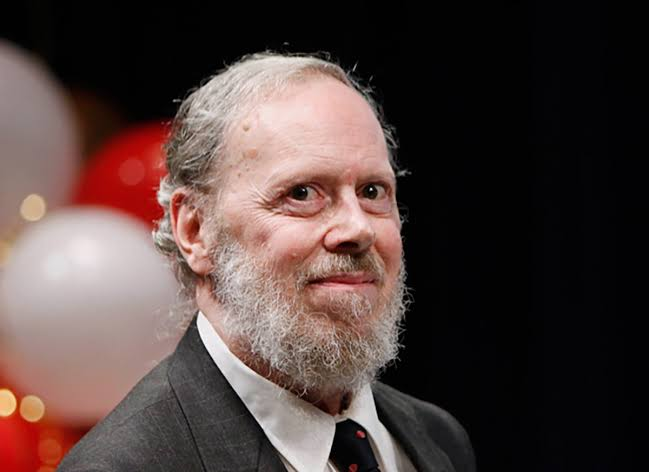
\includegraphics[width=0.5\linewidth]{D.R.png}
  \caption{Dennis Ritchie}
  \label{fig:etiqueta}
\end{figure}

\vspace{5pt}
\subsection*{Nacimiento y Educación}

\textbf{Fecha y Lugar de Nacimiento}: Nació en Bronxville, Nueva York, el 9 de septiembre de 1941.

\textbf{Educación}: Obtuvo dos grados en física y matemática aplicada.

\subsection*{ Carrera Profesional}
\begin{itemize}


  \item \textbf{Década de 1960}: Ritchie y Ken Thompson trabajaron en el sistema operativo Multics en los laboratorios Bell. Thompson encontró una vieja máquina PDP-7 y desarrolló programas de aplicación y un sistema operativo desde cero, con la ayuda de Ritchie y otros.
  \item \textbf{1970}: Brian Kernighan sugirió el nombre "Unix", un juego de palabras con "Multics". Thompson creó el lenguaje B, que luego fue reemplazado por C, creado por Ritchie.
  \item  \textbf{Desarrollo de Unix y C}: Ritchie siguió contribuyendo al desarrollo de Unix y C durante muchos años.
\end{itemize}
\subsection*{ Aportes Importantes}
\begin{itemize}



  \item \textbf{Lenguaje de Programación C}: Ritchie es conocido sobre todo por ser el creador del lenguaje de programación C, uno de los lenguajes de programación más influyentes y utilizados en el mundo.
  \item \textbf{Sistema Operativo Unix}: Ritchie, junto con Ken Thompson, fue el cocreador del sistema operativo Unix, que ha tenido un impacto duradero en el desarrollo de sistemas operativos modernos.
  \item \textbf{Manual "El Lenguaje de Programación C"}: Coautor junto con Brian Kernighan del manual "El lenguaje de programación C", conocido como K&R C. Este libro fue el estándar de facto del lenguaje hasta la aparición del ANSI C.
\end{itemize}
\subsection*{ Datos Importantes}
\begin{itemize}
  \item \textbf{Colaboración con Ken Thompson}: Su trabajo con Ken Thompson en Multics y Unix sentó las bases para muchos desarrollos tecnológicos posteriores.

  \item \textbf{Impacto del Lenguaje C}: El lenguaje C ha sido fundamental en el desarrollo de software y sistemas operativos, y sus descendientes directos, como C++, siguen siendo ampliamente utilizados.

  \item \textbf{Reconocimiento Póstumo}: Tras su fallecimiento, el historiador Paul E. Ceruzzi y su colega Brian Kernighan destacaron su legado y la relevancia de sus contribuciones. Kernighan comentó que Ritchie nunca esperó que el C alcanzara tanta relevancia, y destacó que "Las herramientas que Dennis construyó - y sus descendientes directos - hacen funcionar prácticamente todo hoy en día."
\end{itemize}

\newpage
\subsection{{\bfseries Biografía Linus Torvalds}}
\begin{figure}[htb]
  \centering
  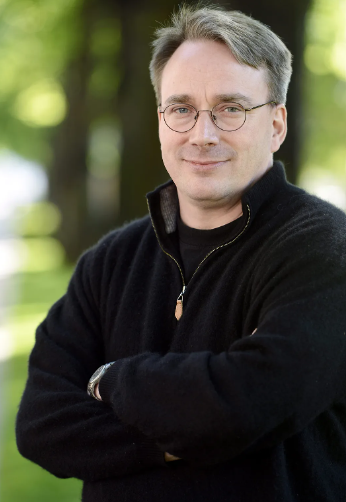
\includegraphics[width=0.3\linewidth]{L.T.png}
  \caption{Linus Torvalds}
  \label{fig:etiqueta}
\end{figure}
\vspace{5pt}
\section*{Historia}
\subsection*{Inicios y Educación}
Linus Benedict Torvalds nació el 28 de diciembre de 1969 en Helsinki, Finlandia. Proviene de una familia intelectual; su padre Nils y su madre Anna Torvalds eran periodistas. Su interés por la computación comenzó a una edad temprana, impulsado por la influencia de su abuelo, quien era profesor de estadística en la Universidad de Helsinki. Linus asistió a la Universidad de Helsinki entre 1988 y 1996, donde se graduó con una maestría en ciencias de la computación.

\subsection*{Desarrollo de Linux}
El desarrollo del sistema operativo Linux comenzó en 1991 mientras Torvalds era un estudiante universitario. Inicialmente, Torvalds buscaba una alternativa a los sistemas operativos existentes, insatisfecho con Minix y sin poder costear una versión comercial de Unix. En la primavera de 1991, comenzó a trabajar en un núcleo (\textit{kernel}) basado en Unix para computadoras con microprocesadores Intel. Una vez completado, Torvalds decidió compartir su creación con la comunidad a través de un servidor FTP, permitiendo a otros contribuir y mejorar el sistema.

\subsection*{Aportes Importantes}
\subsubsection*{Creación del Núcleo Linux}
Linus Torvalds es más conocido por crear el núcleo Linux, que se convirtió en la base de numerosas distribuciones de sistemas operativos. Originalmente llamado \textit{Freax} (una combinación de \textit{free}, \textit{freak} y \textit{x} en referencia a Unix), el nombre fue cambiado a \textit{Linux} por el administrador del servidor donde Torvalds publicó el código. El núcleo Linux, lanzado bajo la Licencia Pública General de GNU, permitió que muchas compañías y desarrolladores individuales crearan sus propias versiones del sistema operativo, conocidas como distribuciones.

\subsubsection*{Impacto en la Tecnología}
El impacto de Linux ha sido significativo en el mundo de la tecnología. El sistema operativo ha crecido en popularidad y uso, desde servidores web hasta dispositivos móviles (como el sistema operativo Android, que se basa en Linux), supercomputadoras y sistemas embebidos. La naturaleza abierta y colaborativa de su desarrollo ha promovido una cultura de innovación y ha puesto en riesgo la primacía de sistemas operativos comerciales como Windows de Microsoft.

\subsection*{Datos Importantes}
\begin{itemize}
  \item Licencia Pública General: Linux se distribuye bajo la Licencia Pública General de GNU (GPL), lo que permite a cualquiera usar, modificar y distribuir el software.
  \item Distribuciones de Linux: Varias compañías y comunidades han creado distribuciones de Linux, como Ubuntu, Fedora, Debian, y Red Hat, entre otras, todas basadas en el núcleo original creado por Torvalds.
  \item Reconocimientos: Torvalds ha recibido numerosos premios y honores por su contribución a la computación, incluido el Premio Millennium Technology en 2012.
\end{itemize}
Linus Torvalds continúa siendo una figura influyente en el desarrollo de software libre y de código abierto, supervisando el mantenimiento y la evolución del núcleo Linux.

\newpage
\subsection{{\bfseries Biografía Richard Stallman}}

\begin{figure}[htb]
  \centering
  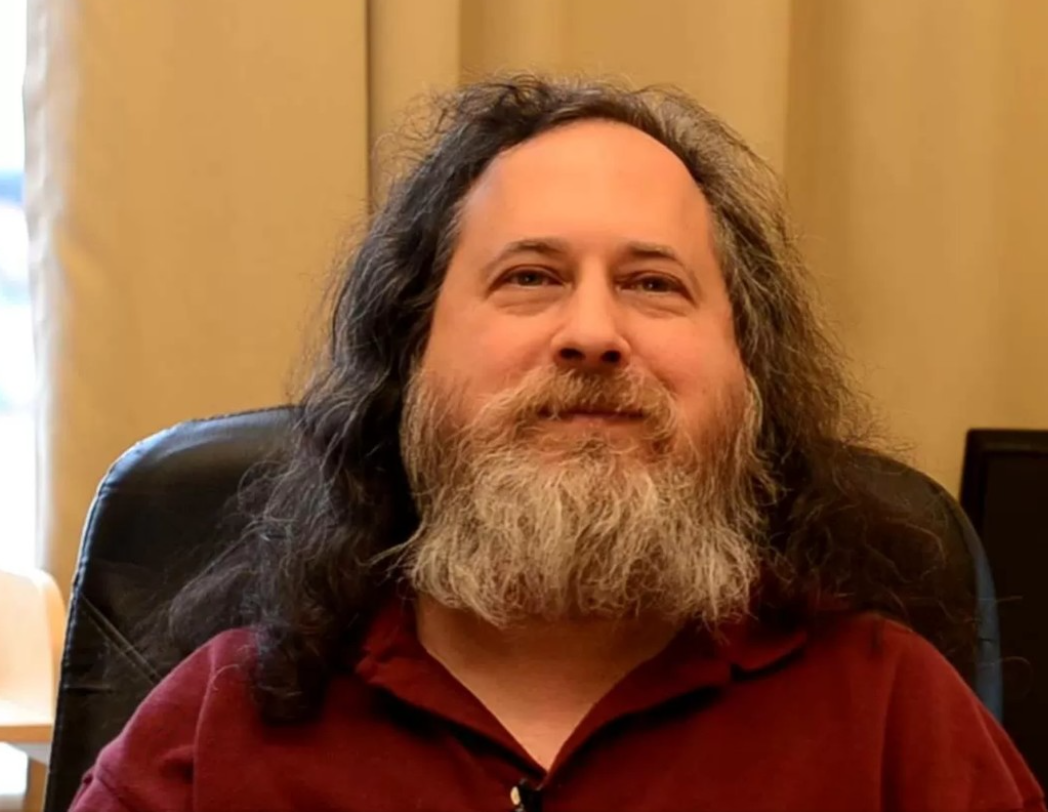
\includegraphics[width=0.5\linewidth]{R.S.1.png}
  \caption{Richard Stallman}
  \label{fig:etiqueta}
\end{figure}
\vspace{5pt}
\textbf{Historia}

Richard Matthew Stallman nació en Manhattan, Nueva York, el 16 de marzo de 1953. Es un destacado programador estadounidense y el fundador del movimiento por el software libre en el mundo. Desde joven, mostró un gran interés por la informática y la programación, lo que lo llevó a estudiar física en la Universidad de Harvard y luego a trabajar en el laboratorio de inteligencia artificial del MIT (Instituto Tecnológico de Massachusetts).

En 1984, Stallman fundó el proyecto GNU (\textit{GNU's Not Unix}) con el objetivo de desarrollar un sistema operativo completamente libre, que pudiera ser utilizado, modificado y redistribuido por cualquier persona. Este proyecto nació como respuesta a la creciente tendencia de las empresas de software a imponer restricciones sobre el uso de sus productos.

\textbf{Aportes Importantes}

\begin{enumerate}
  \item Proyecto GNU y GNU/Linux: Stallman inició el proyecto GNU con la intención de crear un sistema operativo libre. Aunque el núcleo original de GNU no se completó, su combinación con el kernel Linux, desarrollado por Linus Torvalds en 1991, dio lugar a lo que se conoce hoy como GNU/Linux. Este sistema operativo ha sido fundamental para la expansión del software libre.

  \item Free Software Foundation (FSF): Stallman es presidente de la Free Software Foundation, una organización sin ánimo de lucro dedicada a promover y defender el software libre. La FSF ha jugado un papel crucial en la creación de licencias de software libre y en la educación sobre los derechos de los usuarios de software.

  \item Desarrollo de Software: Stallman ha creado varias piezas de software esenciales, incluyendo el editor de texto Emacs, el depurador de software GDB y el compilador GCC (\textit{GNU Compiler Collection}). Estas herramientas son ampliamente utilizadas en la programación y han tenido un impacto significativo en el desarrollo de software.

  \item Concepto de Copyleft y Licencia GPL: Stallman ideó el concepto de "copyleft", que utiliza las leyes de derechos de autor para asegurar que el software libre permanezca libre. Redactó la Licencia Pública General de GNU (GPL), que permite a los usuarios copiar, modificar y redistribuir el software libre bajo ciertas condiciones. La GPL es una de las licencias de software libre más utilizadas en el mundo.
\end{enumerate}

\textbf{Datos Importantes}

\textit{Premios y Reconocimientos}
\begin{itemize}

  \item En 1990, Stallman recibió la beca de la MacArthur Foundation.
  \item En 1991, recibió el premio Grace Hopper de la Association for Computing Machinery (ACM) por el desarrollo de Emacs.
  \item En 1996, fue galardonado con el doctorado honorario del Instituto Real de Tecnología de Suecia.
  \item En 1998, recibió el premio Pioneer de la Electronic Frontier Foundation junto con Linus Torvalds.
  \item En 1999, se le otorgó el premio Yuri Rubinski.
\end{itemize}
\textit{Contribución al Desarrollo de Linux}

En 1991, Linus Torvalds comenzó a escribir el núcleo Linux y decidió distribuirlo bajo la licencia GPL de Stallman. Este paso permitió que múltiples programadores colaboraran en el desarrollo de Linux, haciendo posible la creación de un sistema operativo libre y funcional al combinar el núcleo Linux con el sistema GNU, conocido hoy como GNU/Linux.

\textit{Filosofía del Software Libre}

Stallman es conocido por su firme postura sobre la libertad del software. Afirma que "el software libre es una cuestión de libertad: la gente debería ser libre de usar el software de todas las formas consideradas socialmente útiles". Esta filosofía ha influido profundamente en la forma en que se desarrolla y distribuye el software en todo el mundo.

\subsection*{Bibliografía}
\begin{itemize}
  \item \textbf{Referencias: Richard Stallman - Edad, ciudad natal, biografía | Last.fm.} (s. f.). Last.fm. \url{https://www.last.fm/es/music/Richard+Stallman/+wiki}

  \item \textbf{Wikiwand - Richard Stallman.} (s. f.). Wikiwand. \url{https://www.wikiwand.com/es/Richard_Stallman}

  \item \textbf{Wikiwand - Linus Torvalds.} (s. f.). Wikiwand. \url{https://www.wikiwand.com/es/Linus_Torvalds}

  \item \textbf{Wikiwand - Dennis Ritchie.} (s. f.). Wikiwand. \url{https://www.wikiwand.com/es/Dennis_Ritchie}

  \item \textbf{Dergarabedian, C.} (2023, 12 marzo). Quién fue Dennis Ritchie, el creador de una tecnología que usás a diario y que influyó más que Steve Jobs. iProfesional. \url{https://www.iprofesional.com/tecnologia/378220-dennis-ritchie-el-creador-de-una-tecnologia-que-usas-a-diario}
\end{itemize}
\newpage
\section{Consulta 2}
\subsection{Arquitectura Android}

Android es un sistema operativo móvil desarrollado por Google. Desde su lanzamiento en 2008, se ha convertido en uno de los sistemas operativos móviles más populares del mundo, con una gran cantidad de dispositivos que ejecutan Android en todo el mundo.

La arquitectura de Android se basa en un sistema operativo Linux y está compuesta por varias capas y componentes que trabajan juntos para proporcionar la funcionalidad del sistema. Estas capas incluyen:
\begin{itemize}


  \item Capa de Aplicaciones: Esta capa alberga las aplicaciones instaladas en el dispositivo. Las aplicaciones pueden ser desarrolladas por terceros o por el propio fabricante del dispositivo.

  \item Capa de Marco de Trabajo: Esta capa proporciona herramientas y APIs para el desarrollo de aplicaciones. Incluye componentes como el Administrador de Actividades, el Administrador de Recursos y el Administrador de Ventanas.

  \item Capa de Bibliotecas: Esta capa contiene bibliotecas de código que proporcionan funcionalidades adicionales a las aplicaciones. Incluye bibliotecas como SQLite (para el almacenamiento de datos), OpenGL ES (para gráficos 2D y 3D) y WebKit (para navegación web).

  \item Capa de Kernel: Esta capa se encarga de administrar los recursos del hardware, como la memoria, el procesador y los controladores de dispositivos. Utiliza el kernel de Linux como base.
\end{itemize}
Esta arquitectura modular de Android permite un desarrollo flexible y personalizado de aplicaciones, al tiempo que proporciona una experiencia de usuario coherente en diferentes dispositivos.

\subsection{Arquitectura iOS}
La arquitectura de iOS se compone de varias capas principales que trabajan juntas para proporcionar un entorno operativo completo y eficiente. Estas capas incluyen:
\begin{itemize}
  

  \item Capa Cocoa Touch: Esta capa es responsable de la interacción del usuario y proporciona la mayoría de las interfaces de usuario de iOS. Incluye frameworks como UIKit (para la interfaz de usuario) y Core Animation (para animaciones).

  \item Capa de Medios: Esta capa proporciona soporte para gráficos, audio y video. Incluye frameworks como Core Graphics (para gráficos vectoriales), Core Audio (para audio digital) y AV Foundation (para reproducción de video).

  \item Capa de Servicios Centrales: Esta capa proporciona servicios esenciales para las aplicaciones, como el acceso a la red, la gestión de archivos y la detección de ubicación. Incluye frameworks como Foundation (para la gestión de datos), Core Location (para la detección de ubicación) y CloudKit (para el almacenamiento en la nube).

  \item Capa de Sistema Operativo Central: Esta capa incluye componentes del sistema operativo iOS, como el administrador de memoria, el administrador de energía y el administrador de tareas.

  \item Núcleo y Controladores de Dispositivos: Esta capa está directamente relacionada con el hardware y proporciona controladores de dispositivos para el funcionamiento del dispositivo.
\end{itemize}
La arquitectura de iOS se caracteriza por su integración estrecha entre hardware y software, lo que contribuye a una experiencia de usuario fluida y una alta seguridad.

\subsection{Arquitectura macOS}
El sistema operativo macOS se basa en el kernel de Darwin, que a su vez se basa en UNIX. Darwin es la base del sistema operativo macOS actual. Aunque Darwin es de código abierto, la última versión del sistema operativo macOS es una versión propietaria llamada macOS Ventura, que se lanzó al público en octubre de 2022.
La arquitectura de macOS se compone de las siguientes capas:
\begin{itemize}
  \item Capa de Aplicaciones: Esta capa alberga las aplicaciones y servicios del sistema. Incluye aplicaciones como Mail, Safari y iTunes, así como servicios como Time Machine y iCloud.

  \item Capa del Entorno de Utilización: Esta capa proporciona herramientas y APIs para el desarrollo de aplicaciones en macOS. Incluye frameworks como Cocoa (para la interfaz de usuario) y Core Services (para servicios comunes como el acceso a archivos y la gestión de procesos).

  \item Capa del Núcleo: Esta capa se encarga de administrar los recursos del hardware, como la memoria, el procesador y los controladores de dispositivos. Utiliza el kernel de Darwin como base.


  \item apa de Servicios Centrales: Esta capa proporciona servicios esenciales para las aplicaciones en macOS, como el acceso a la red, la gestión de archivos y la detección de ubicación. Incluye frameworks como Foundation (para la gestión de datos), Core Services (para servicios básicos del sistema) y CloudKit (para el almacenamiento en la nube).

  \item Capa del Núcleo del Sistema Operativo: Esta capa contiene el núcleo del sistema operativo macOS, que proporciona funcionalidades básicas como la administración de procesos, la gestión de memoria y la administración de dispositivos de hardware. También se encarga de asegurar la estabilidad y seguridad del sistema.
\end{itemize}
La arquitectura de macOS se beneficia de la base de código abierto de Darwin, que proporciona una sólida base de sistema operativo UNIX. Además, macOS se destaca por su interfaz gráfica de usuario intuitiva y su integración con otros dispositivos y servicios de Apple, lo que brinda una experiencia de usuario coherente en el ecosistema de Apple.
\vspace{5pt}
\subsection*{Bibliografía}
\begin{itemize}
  \item \textbf{Revelo, J.} (2020, 30 noviembre). Aprendiendo sobre la arquitectura de Android. Develou. \url{https://www.develou.com/aprendiendo-la-arquitectura-de-android/}

  \item \textbf{Prezi, A. C. C. O.} (s. f.).Arquitectura del sistema operativo Mac. prezi.com. \url{https://prezi.com/bdly6ld-kc6b/arquitectura-del-sistema-operativo-mac/#:~:text=El%20Mac%20OS%20X%20posee,la%20interfaz%20de%20usuario%20Aqua.}

  \item \textbf{Prezi, C. R. O.} (s. f.). Arquitectura IOS. prezi.com. \url{https://prezi.com/srjcjo5pb5uu/arquitectura-ios/}
\end{itemize}

\end{document}